\documentclass[a4paper,11pt,openright,oneside]{report}
\usepackage[utf8]{inputenc}
\usepackage[margin=2cm]{geometry}
\usepackage[T1]{fontenc}
\usepackage[portuguese]{babel}
\usepackage{graphicx}
\usepackage{csquotes}
\usepackage{blindtext}
\usepackage[printonlyused]{acronym}
\usepackage{hyperref}
\usepackage[titletoc,title]{appendix}
\usepackage{caption}
\usepackage{subcaption}
\newcommand{\RNum}[1]{\uppercase\expandafter{\romannumeral #1\relax}}

\begin{document}

\title{\textbf{Comando Infra-Vermelhos no Controlo de LEDs}\\[1cm]\textsc{\small {Departamento de Electrónica, Telecomunicações e Informática} \\ \large {UNIVERSIDADE DE AVEIRO}}}
\author{Sandra Moreira 76471, Ricardo Jesus 76613\\simoreira@ua.pt, ricardojesus@ua.pt}
\date{1 de Junho de 2015}
\maketitle
\pagenumbering{arabic}

\chapter{Infra-Vermelhos no Controlo de LEDs}

\section{Introdução}
\label{sec:introdução}

No âmbito da unidade curricular de Laboratórios de Sistemas Digitais, foi proposto o desenvolvimento de um mini-projeto relativo aos conteúdos abordados ao longo do semestre. Neste sentido, foi desenvolvido um módulo de infra-vermelhos que permite controlar várias componentes do KIT DE2-115 da Terasic através do comando que o acompanha, de acordo com o tema apresentado e escolhido no guião de propostas. Desta forma a partir do comando deverá ser possível controlar o número de LEDs verdes acesos do KIT, bem como a sua intensidade luminosa, em função da tecla premida.

\section{Arquitetura do Sistema}
\label{sec:arquitetura}

De acordo com o projeto escolhido, o desenvolvimento focou-se na parte essencial deste, ou seja, a receção e descodificação de códigos infra-vermelhos. Desse modo, foi implementado o bloco Recetor de IR, responsável por receber o código referente à tecla premida enviado pelo comando e transmiti-lo para o resto da máquina. Assim, esse código chega ao bloco controlador de ações que decide se este é responsável por definir o número de LEDs verdes acesos ou por controlar a luminosidade destes. Se o valor de 8 bits for referente a este último, será também processado o número de LEDs vermehos acesos e o valor a mostrar nos mostradores hexadecimais.
No primeiro caso apenas se ligarão o número de LEDs verdes equivalente ao número premido no comando. Caso tenha sido alterada a luminosidade, o código passará, então, para o bloco contador de PWM. Neste bloco, é mantido o registo do valor de luminosidade em uso e é ajustado conforme indicado: adicionando ou subtraindo uma unidade ao valor atual, guardando este valor e colocando a luminosidade a zero (ou vice-versa, caso seja premida a tecla de \textit{Power Off}), ou simplesmente mantendo este valor sem alterações. Posto isto, é enviado um código de 4 bits para o bloco PWM que controla a intensidade luminosa dos LEDs verdes. Foi também implementado um bloco de som que, quando tanto o número de LEDs verdes acesos como a sua luminosidade está no máximo, emite um som de alerta. Por último, foi também decidido implementar um bloco que permitisse mostrar no LCD da FPGA os desenvolvedores deste projeto.

O diagrama de blocos presente na figura \ref{fig:ir_leds0} ilustra a implementação acima, apesar de existirem blocos considerados muito simples (e que constituem outros blocos) que foram omitidos de forma a não se sobrecarregar o diagrama.

\begin{figure}[ht]
\center
\fbox{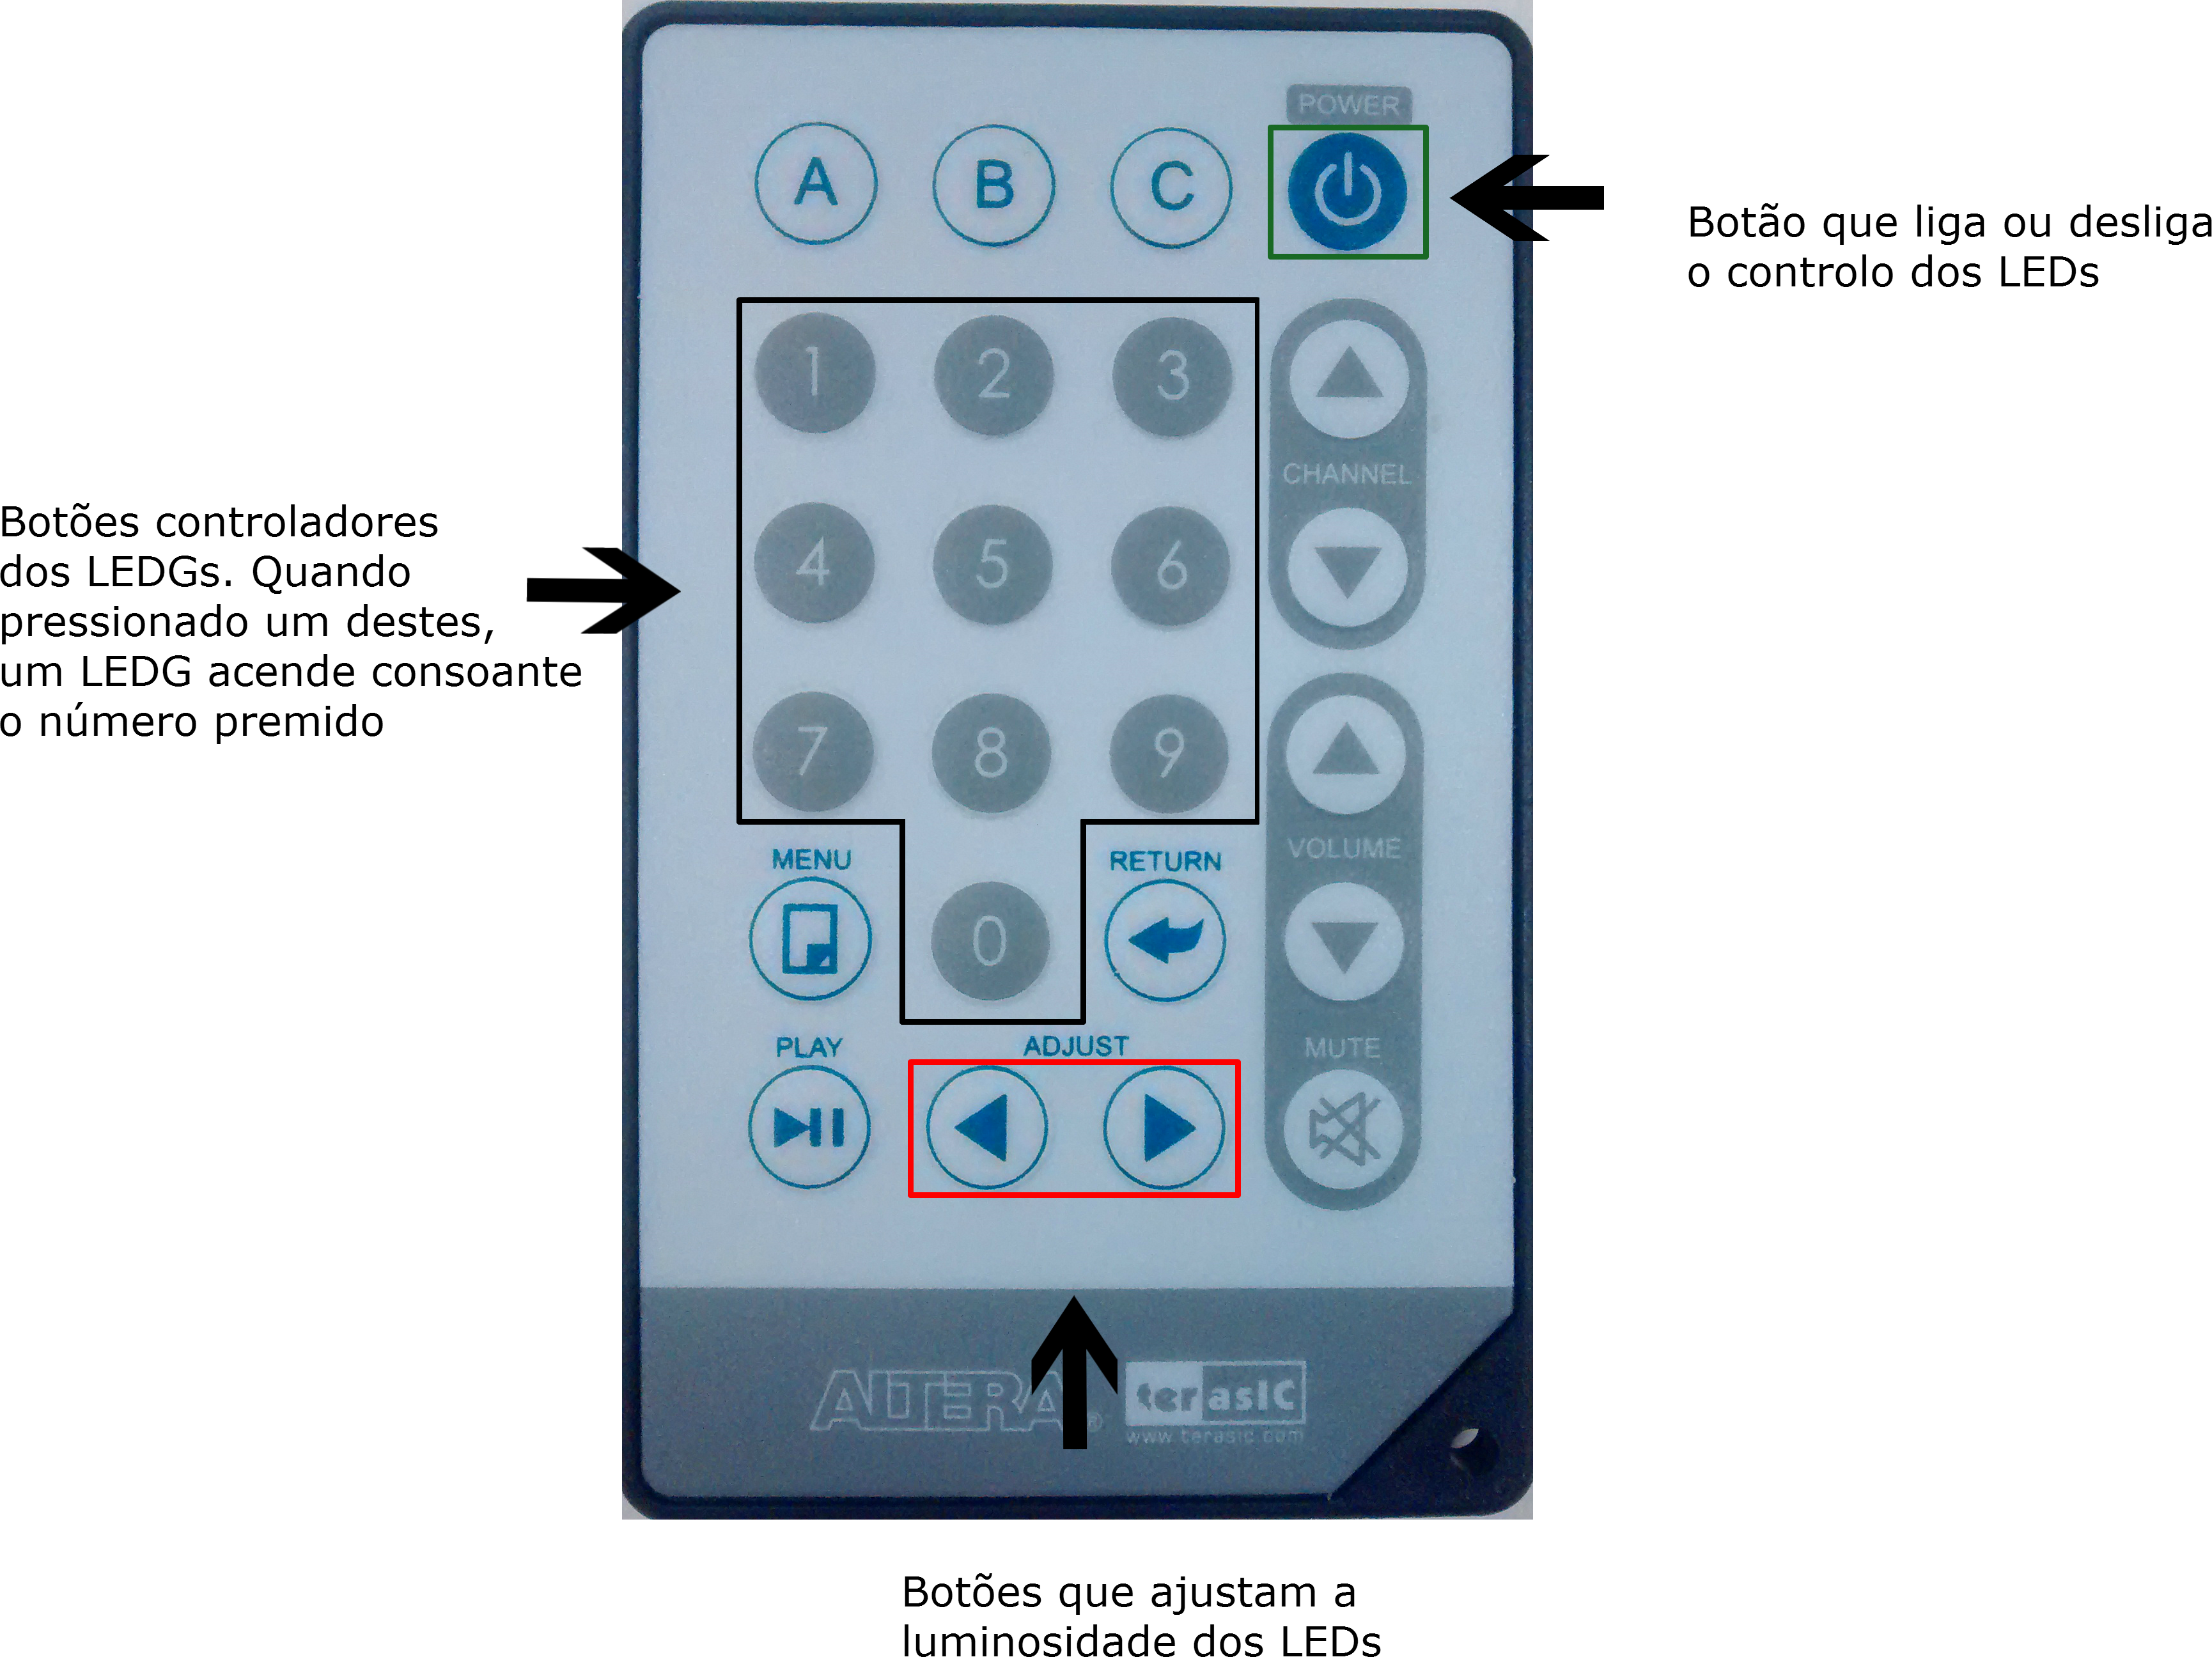
\includegraphics[height=7cm]{img/ir_leds0}}
\caption{Diagrama de blocos do sistema implementado}
\label{fig:ir_leds0}
\end{figure}

Assim, o sinal de infra-vermelhos deverá ser recebido pelo bloco recetor de IR e, em função da tecla premida, deverão ser ajustados ou a intensidade luminosa dos LEDs verdes ou o número destes LEDs acesos. Todas os outros valores da FPGA serão atualizados/ajustados em função destes dois.

\section{Implementação}
\label{sec:implementação}

\subsection*{Recetor Infra-Vermelhos}

Este bloco recebe o sinal de infra-vermelhos (\verb|irda_rxd|) do kit, tendo como objetivo realizar uma amostragem deste, permitindo assim determinar que tecla do comando foi premida. Para isso teve-se em conta as seguintes especificações (obtidas de \url{ftp://ftp.altera.com/up/pub/Altera_Material/13.1/Boards/DE1-SoC/DE1_SoC_User_Manual.pdf}, p.75):
\begin{description}
\item[Start Bit] Bit enviado de forma a marcar o início do envio de informação

9ms nível lógico '0' $\rightarrow$ 4.5ms nível lógico '1'
\item[Data Bit] 32 bits de informação, a começar no menos significativo

562.5$\mu$s nível lógico '0' $\rightarrow$ 562.5$\mu$s nível lógico '1': '0' lógico\\
562.5$\mu$s nível lógico '0' $\rightarrow$ 1.6875ms nível lógico '1': '1' lógico

\item[Stop bit] Bit que denota o final do código

562.5$\mu$s nível lógico '0'
\end{description}

Para além disso, dos 32 bits que compõem o código transmitido apenas os dos índices 23 ao 16 representam a tecla premida, sendo os últimos 8 (31 até 24) a negação lógica destes. Isto é importante já que permite verificar com alguma segurança que não se cometeram erros ao amostrar o sinal.

Assim, implementou-se a máquina de estados exposta na figura \ref{fig:ir_leds1} e que acenta maioritariamente em quatro contadores referentes ao tempo de cada nível lógico. Isto foi possível já que conhecendo-se a frequência do sinal de relógio utilizado (50MHz), calculou-se o período deste (20ns) e assim determinaram-se valores ``meta'' que os contadores devem atingir para transitar de estado. Todos eles foram definidos com alguma margem de erro face ao exposto acima, de forma a combater possíveis ruídos de hardware. Procurou retratar-se as seguintes três fases de receção de um código:

\begin{description}
\item[IDLE] Este é o estado inicial da máquina. Neste estado, espera-se por que o sinal de \verb|irda_rxd| comute para '0'. Quando isso acontece, é iniciado um contador que deve contar por 4.6ms (face aos 9ms indicados, pelas razões explicadas acima). Quando \verb|irda_rxd| comuta para '1', e tendo sido atingido o valor definido para este contador, então transita-se para o estado \textit{Guidance};
\item[Guidance] Estado em que se confirma se o \texttt{start bit} é o esperado. Assim, inicia-se um contador que deve contar por 4.2ms, enquanto \verb|irda_rxd| se encontra a '1'. Caso este objetivo seja atingido, então o estado comuta para \textit{DataRead};
\item[DataRead] Neste estado são lidos bit a bit os 32 bits transmitidos. Para isso tenta contar-se por 0.83ms o valor lógico '1', sendo que quando este contador conta 0.4ms o indíce do vetor do bit que se está a amostrar é incrementado. Assim, caso o contador atinga os 0.83ms considera-se o bit como sendo um '1' lógico, caso contrário mantém-se como '0'. No final, quando são lidos 32 bits, verifica-se se os penúltimos 8 são a negação lógica dos últimos 8. Caso sejam, o vetor de saída é atualizado e a saída \verb|DataReady| posta temporariamente a '1', indo-se depois para o estado \verb|IDLE|. Caso contrário, transita-se imediatamente para \verb|IDLE|.
\end{description}

\subsection*{Controlo de Ações}

Entidade responsável por ou definir o número de LEDs verdes acesos, ou ajustar a intensidade destes, ou ainda colocar o sistema num estado de \textit{Power Off}. Para isso comunica com os blocos \verb|PWM Counter| e \verb|LengthSetter|, fornecendo-lhes os devidos valores.

\subsection*{PWM Counter}

Bloco que mantém registo do valor de PWM num dado instante, sendo capaz de o incrementar ou decrementar. Faz uso de um divisor de frequência de forma a garantir que os valores não sofrem alterações bruscas (por exemplo de 0 para 10).

\subsection*{PWM}

Bloco responsável por gerar um sinal que comuta entre '0' e '1' lógicos de forma a simular resultados que seriam de outra forma obtidos de forma analógica (por exemplo com alteração de voltagem fornecida). Isto permite de facto controlar a intensidade luminosa dos LEDs verdes. Para tal, é estabelecido uma frequência para o sinal a gerar (foi escolhido 10kHz). De seguida, de acordo com a resolução definida em ``compile time'' (no caso deste projeto, de 4 bits) e com o valor introduzido nas entradas do bloco, é definido até que instante do período deve o sinal de saída estar a '1'. Após esse tempo, o sinal comuta para '0', sendo depois o ciclo repetido. É de notar que a visão humana não reage à intensidade luminosa de uma forma tão linear quanto o realizado por esta implementação, e portanto em valores baixos de PWM serão notadas grandes alterações, ao contrário de valores mais elevados em que parece não ser registada nenhuma diferença.

\subsection*{Mostrador de PWM em LEDRs}

Bloco que mostra o valor de PWM de um instante nos LEDs vermelhos da FPGA, desde que pelo menos um LED verde esteja aceso (e o valor de PWM seja 1). Devido ao exposto no final de \verb|PWM| escolheu-se inicialmente incrementar/decrementar os LEDs acesos por duas unidades. A partir do valor 3, os ajustes deverão ser de uma unidade apenas.

\subsection*{Descodificador de 4 bits para HEX5 e HEX4}

Este bloco deve receber o valor de PWM do instante atual, e mostrá-lo nos displays hexadecimais (HEX5 e HEX4) da FPGA, em base decimal, onde HEX5 regista as dezenas e HEX4 as unidades.

\subsection*{Definir LEDGs acesos}

Bloco que deve definir o número de LEDs verdes acesos. O máximo será 9, o mínimo 0.

\subsection*{Unidade de LCD}

Bloco que mostrará no LCD da FPGA uma imagem estática com os nomes de quem desenvolveu este projeto. Esta interface não foi desenvolvida (mas apenas ajustada) pelos autores deste documento. A sua implementação assentou no projeto disponibilizado pelo prof. Bernardo Cunha.

\subsection*{Interface de Áudio}

Este bloco deve permitir que quando os 9 LEDs verdes estiverem acesos com a intensidade máxima (valor de PWM 15), deverá ouvir-se um bip sonoro. Tal como o módulo anterior, a implementação deste bloco baseou-se na disponibilizada pelos docentes da U.C., tendo apenas sido realizados ajustes para a tornar funcional neste projeto.

\begin{figure}[ht]
\center
\fbox{\includegraphics[height=7cm]{img/ir_leds1}}
\caption{Diagrama de estados do bloco recetor de Infra-Vermelhos}
\label{fig:ir_leds1}
\end{figure}

\section{Validação de Resultados}
\label{sec:validação}

A maioria dos blocos desenvolvidos foram submetidos a alguma forma de validação, salvaguardando-se blocos muito simples ou que foram disponibilizados pelos docentes da U.C.. Na figura \ref{fig:testbenches} são expostos os resultados obtidos para os blocos recetor de infra-vermelhos e gerador do sinal modulado (PWM), blocos considerados fundamentais dado o enunciado do projeto.

\begin{figure}
        \centering
        \begin{subfigure}[b]{1\textwidth}
                \includegraphics[width=\textwidth]{img/ir_leds2}
                \caption{Testbench de recetor de infra-vermelhos}
                \label{fig:ir_leds2}
        \end{subfigure}

        \begin{subfigure}[b]{1\textwidth}
                \includegraphics[width=\textwidth]{img/ir_leds3}
                \caption{Testbench de bloco PWM}
                \label{fig:ir_leds3}
        \end{subfigure}
        \caption{Alguns testes obtidos através do software ModelSim da Altera}\label{fig:testbenches}
\end{figure}

Na figura \ref{fig:ir_leds2} é visível como o bloco recetor de IR é de facto capaz de amostrar o sinal que seria enviado caso a tecla \textit{A} do comando fosse premida. A correta receção de todos os outros códigos do comando foi realizada recorrendo-se diretamente à FPGA, onde o código recebido foi mostrado nos LEDs verdes, sendo depois comparado com os valores indicados na documentação do comando. Escolheu-se esta abordagem para evitar escrever uma testbench com centenas de linhas de código (tornando-a extremamente confusa), quando à partida se o algoritmo usado funciona para uma situação então deve funcionar para todos os casos.

Por outro lado, na figura \ref{fig:ir_leds3} é visível a modulação gerada. Inicialmente o sinal gerado tem um duty-cycle que ronda os 0\%, enquanto que para o valor máximo (15, com 4 bits de resolução), este valor ronda os 100\%.

\section{Conclusão}
\label{sec:conclusão}

Este projeto permitiu que interagíssemos tanto com temas abordados ao longo do semestre como com outros que nos obrigaram a procurar e aprender por nós próprios. Veja-se como fomos obrigados a procurar sobre como interagir com o sensor de IR da FPGA, lendo dele sinais enviado por outra fonte, face ao desenvolvimento de testbenches, tema abordado pela U.C.. Contudo, apesar dos infra-vermelhos terem sido um assunto complicado mas interessante de se entender e implementar, consideramos que o projeto se focaria em demasia em assuntos pouco abordados na U.C. (pelo menos para os blocos fundamentais do sistema) e, por isso, de forma a tentar conjugar um pouco os vários conteúdos abordados ao longo do semestre, consideramos que seria enriquecedor adicionar módulos utilizando som e o LCD do kit, de forma a completar e a dinamizar o nosso trabalho.

Em suma, consideramos esta proposta interessante e capaz de desenvolver melhor as temáticas tratadas durante as aulas. Sentimos que o nosso objetivo foi alcançado e que o nosso projeto cumpre aquilo que foi pensado inicialmente.

\section{Manual de Utilizador}

Através do comando de infra-vermelhos que acompanha o kit DE2-115 deverá ser possível definir o número de LEDs verdes acesos, valor que varia de 0 a 9, bem como a intensidade luminosa destes, valor compreendido entre 0 e 15. A intensidade luminosa dos LEDs deve ser mostrada nos LEDs vermelhos, que funcionam como uma barra que se vai enchendo (ou seja, os LEDs vão acendendo) conforme a intensidade aumenta, bem como nos HEX5 e HEX4 da FPGA, onde é imprimido o valor em base decimal. O botão de \textit{Power Off} coloca a FPGA num estado de \textit{Standby}, como se efetivamente estivesse ligada/desligada. Quando os 9 LEDs verdes estão acesos e a sua intensidade é 15 ouve-se um bip, indicando que os valores máximos foram atingidos simultaneamente. Por fim, no ecrã LCD deverá ser mostrado quem desenvolveu este projeto. Na figura \ref{fig:ir_leds4} mostra-se quais as teclas do comando a que foram atribuídas funções e quais são estas.

\begin{figure}[ht]
\center
\fbox{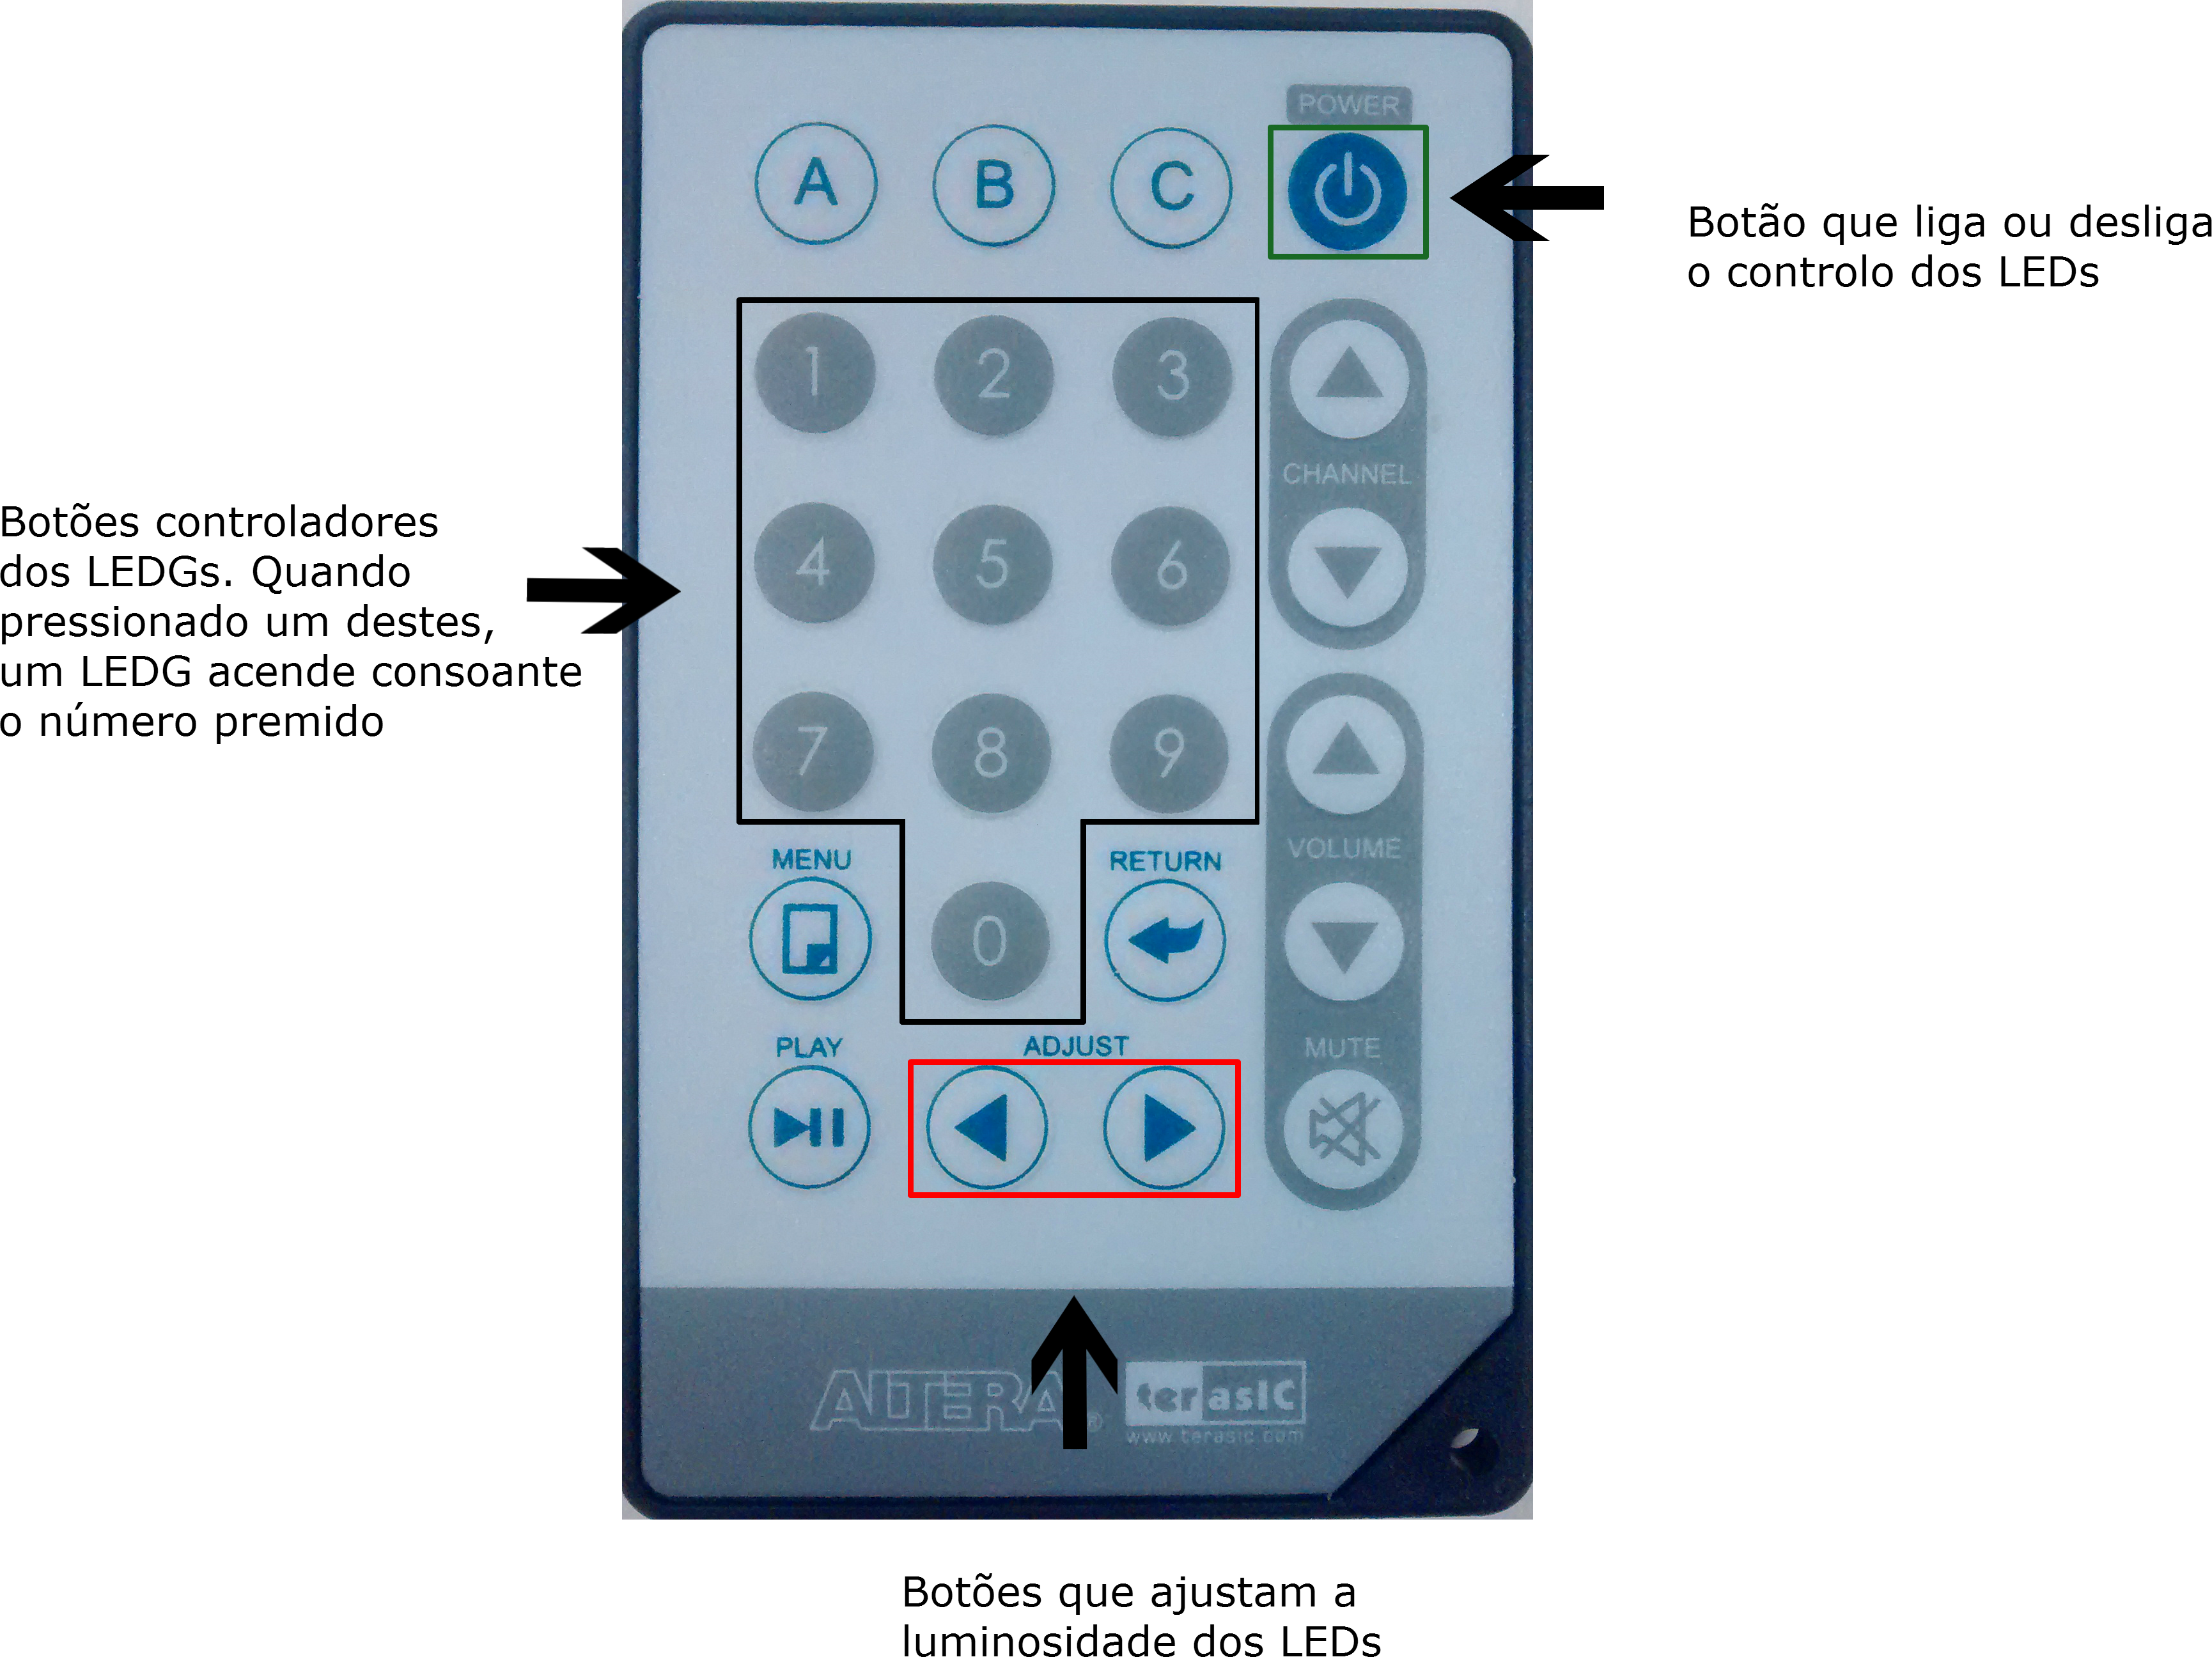
\includegraphics[height=7cm]{img/ir_leds4}}
\caption{Funções do comando utilizado}
\label{fig:ir_leds4}
\end{figure}

\maketitle
\nocite{*}

\end{document}
